\documentclass[10pt,onecolumn,letterpaper]{article}
%% Welcome to Overleaf!
%% If this is your first time using LaTeX, it might be worth going through this brief presentation:
%% https://www.overleaf.com/latex/learn/free-online-introduction-to-latex-part-1

%% Researchers have been using LaTeX for decades to typeset their papers, producing beautiful, crisp documents in the process. By learning LaTeX, you are effectively following in their footsteps, and learning a highly valuable skill!

%% The \usepackage commands below can be thought of as analogous to importing libraries into Python, for instance. We've pre-formatted this for you, so you can skip right ahead to the title below.

%% Language and font encodings
\usepackage[spanish,english]{babel}
\usepackage[utf8x]{inputenc}
\usepackage[T1]{fontenc}

%% Sets page size and margins
\usepackage[a4paper,top=3cm,bottom=2cm,left=3cm,right=3cm,marginparwidth=1.75cm]{geometry}

%% Useful packages
\usepackage{amsmath}
\usepackage{graphicx}
\usepackage[colorinlistoftodos]{todonotes}
\usepackage[colorlinks=true, allcolors=blue]{hyperref}
 \usepackage{float}
%% Title
\title{
		%\vspace{-1in} 	
		\usefont{OT1}{bch}{b}{n}
		\normalfont \normalsize \textsc{MIE 1624 Introduction to Data Science and Analytics} \\ [10pt]
		\huge Assignment 3: Course Curriculum Design \\
}

\usepackage{authblk}

\author{Yunjie Xu 1008601951}


	\affil{\small{Department of Mechanical and Industrial Engineering, University of Toronto}}


\begin{document}
\maketitle

\selectlanguage{english}


%%\begin{abstract}
%%The abstract is probably what you'll be writing last, and should be roughly 300 words in length. Your abstract will get published whether or not your team wins the challenge, so make sure to do an extra good job of it! An easy way to structure your abstract is to write individual summaries of the four parts of your paper (Introduction, Methods, Results, Discussion) and then put them together once you're done.
%%\end{abstract} \\ 
%%\\ 
%%{\textbf{Keywords} \\
%%pick, 3-5, good, keywords}

\section*{Introduction}
For this assignment, the aim is to design an applicable course curriculum in line with the needs of the industry for a new "Master of Business and Management in Data Science and Artificial Intelligence" program at the University of Toronto. The dataset includes more than 1400 job descriptions from Indeed's web scraping. These jobs are all from the North American job market, and the job positions are all Data Analyst or Data Scientist.


\section*{Part 1}
Firstly, I do two web scraping for Data Analyst and Data Scientist separately. Then I combine two sheets, renaming the new sheet as 'webscraping\_results\_assignmnet3.csv'. I only keep the 'Descriptions' and 'Title' columns because data for other columns are mainly missing or difficult to classify, so I drop these columns. Lastly, I drop duplicate jobs, and there are 1452 jobs left.

\section*{Part 2}
\subsection*{a/b}
I separately extract technical/hard skills and business/soft skills by searching for keywords. Then I create a column for each skill. If the description includes this skill, I use the number 1 to represent that the job needs this skill; otherwise, I use the number 0. After finishing this step, the data transform into a logically formatted data structure for clustering analysis 

\subsection*{c/d}
In general, 75\% of all the requirements of the candidate for the enterprise are about hard skills, and the remaining 25\% are about soft skills (Figure 1). For Data Analysts, the proportion of soft skills has reached 31.5\% (DS is 24.1\%), which means that the standards for measuring Data Analysts are more diverse (Figure 2).\\

\noindent from the perspective of skills, the soft skills that companies value most are communication, leadership, research, passion, and innovation (Figure 3). The essential hard skills can be divided into two different types. One is theories, and the other is tools. The critical tools are R, Python, SQL, Visio, Excel, etc. And the curtail theories are about AI, machine learning, statistics, computer science, etc (Figure 4).\\

\noindent On the side of different types of jobs, the job requirements for da are more straightforward; usually, a qualified DA needs to be good at communication, curious, and proficient in using R, Excel, SQL, Visio, etc (Figure 6). However, the requirements of DS are much more complicated. From the perspective of the cloud map, different DS positions have additional requirements, which leads to the fact that most of the words in the cloud map are relatively small and dense. Generally, a good DS should handle R, AI, Python, Statistics, machine learning, and research. In contrast, Excel and SQL are no longer essential tools for DS (Figure 7).The DS position has stricter and more varied technical requirements for candidates, and different positions have different needs in detail. The requirements of the DA position are more straightforward, and recruiters care more about candidates' soft power.

\section*{Part 3}
\subsection*{a/b}
The most challenging thing in this part is to find the distance matrix. I redefine some features by myself. For example, I combine SQL, NoSQL, MySQL, and pgAdmin to the new topic SQL. The advantage of this is that the number of features is significantly reduced. And more importantly, the distance between each feature is not limited to 1 or 0. After integrating features, I deleted the technical skills with frequencies less than 100 and other soft skills that cannot be combined (these are mostly character traits, and it is challenging to design courses to improve). Then I used a method similar to the tutorial to calculate the distance matrix and draw the dendrogram (Figure 8).\\

\subsection*{c}
Based on figure 8, hierarchical clustering can divide the skills into a cluster clearly. I make bullet point to these cluster. 

\begin{itemize}
  \item Cluster 1: Python, R, Deep Learning
  \item Cluster 2: Statistics, Research, Modeling Technology
  \item Cluster 3: Hadoop, Spark, Big data, Java
  \item Cluster 4: Power BI, SAS
  \item Cluster 5: Excel, Visio, Communication
\end{itemize}

\noindent Based on the above results and combined with reality, I designed ten courses for this project. And the result shows below:

\begin{enumerate}
  \item Course 1 : Introduction to Statistical Programming based on R/Python
  \item Introduction to Deep Learning in R/Python
  \item Course 3 : Advanced Statistics for Data Science
  \item Course 4 : Introduction to Statistical Modeling
  \item Course 5 : Introduction to Big Data with Spark and Hadoop
  \item Course 6 : Advanced Big Data with Java
  \item Course 7 : Business Intelligence in Power BI/SAS
  \item Course 8 : Business Practice in Excel/Visio
  \item Course 9 : SQL for Data Science
  \item Course 10 : Building High-Performing Teams and Running Business
\end{enumerate}

\section*{Part 4}
Compared with hierarchical clustering, K-means clustering is not flexible enough because I need to pre-determine how many clusters I want to divide. Thus, I use the elbow method to decided the best number of clusters.The elbow method is a heuristic used in cluster analysis to estimate the number of clusters present in a data set. Plotting the explained variation as a function of the number of clusters, the procedure entails choosing the elbow of the curve as the appropriate number of clusters. From the figure 9, the elbow of curve is 13. However, the maximum number of classes is 12, thus I take 12 as the best number of clusters. And the result shows below:

\begin{itemize}
  \item \textbf{Cluster 1}: Optimization, SAS, Java, Spark, Hadoop, Power BI, Big data \\
        \textbf{Course Name}: Big Data Science with Mutiple Tools
        
  \item \textbf{Cluster 2}: R \\
        \textbf{Course Name}: Introduction to Statistical Porgramming: R
  
  \item \textbf{Cluster 3}: Communication, Visio, Excel\\
        \textbf{Course Name}: Business with Advanced Excel,SQL,and Visio
        
  \item \textbf{Cluster 4}: Statistical Learning \\
        \textbf{Course Name}: Introduction to Statistical Learning
        
  \item \textbf{Cluster 5}: Cloud Computing \\
        \textbf{Course Name}: Cloud Practitioner Essentials
        
  \item \textbf{Cluster 6}: Research, Database, Statistics, Visualization, ERP, Modeling Technology\\
        \textbf{Course Name}: Advanced Statistics and Modeling Technology in Data Science
        
 \item \textbf{Cluster 7}: Team Sprit \\
        \textbf{Course Name}: Building High-Performing Teams
        
 \item \textbf{Cluster 8}: Deep Learning \\
        \textbf{Course Name}: Introduction to Deep Learning
        
 \item \textbf{Cluster 9}: Python \\
        \textbf{Course Name}: Introduction to Statistical Porgramming: Python
        
\item \textbf{Cluster 10}: Data Structure and Algorithm \\
        \textbf{Course Name}: Introduction to Data Structure and Algorithm
        
\item \textbf{Cluster 11}: Commerce Skills\\
        \textbf{Course Name}: Foundations of Commerce
        
\item \textbf{Cluster 12}: SQL \\
        \textbf{Course Name}: SQL for Data Science

\end{itemize}

\noindent Since the number of clusters in k-means clustering is pre-determined, we can see that the number of topics in each cluster is very inconsistent. Some clusters contain only one topic, while others contain many, which is very different from hierarchical clustering. K-means clustering tends to group less relevant topics, which is why some clusters have many topics.

\section*{Part 5}
In the K-means clustering, the project has too many skills, which could make the project design more challenging, and it is also hard for students to properly absorb the abilities they should obtain in one or two semesters. Besides, the course curricula built from hierarchical clustering may better identify business and technical skills and give a curriculum containing both business and technical stream courses. Those two streams of courses supplied can better agree with the program's need to focus on technical and soft skills.\\

\noindent Course curriculums will be shown in the appendix (Figure 10 and Figure 11).

\section*{Appendix}

\appendix

\begin{figure}[H]
  \centering
  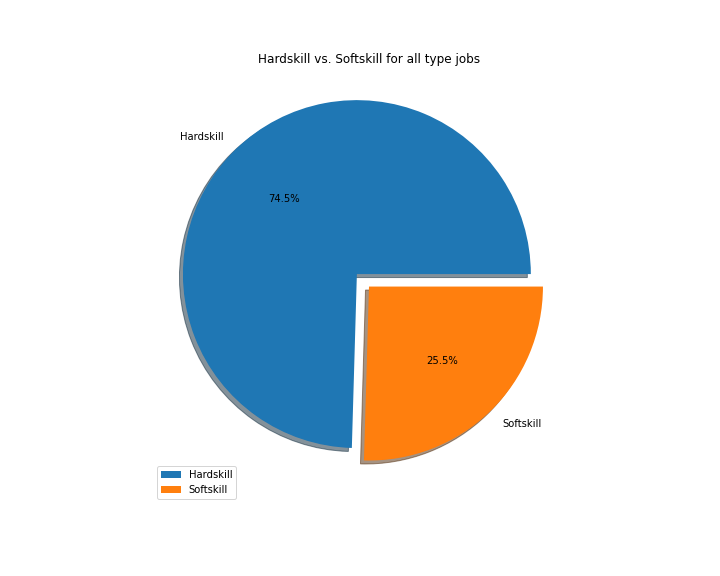
\includegraphics[width=.75\textwidth]{f2.png}
  \caption{'Hardskill vs. Softskill for all type jobs'}
\end{figure}

\begin{figure}[H]
  \centering
  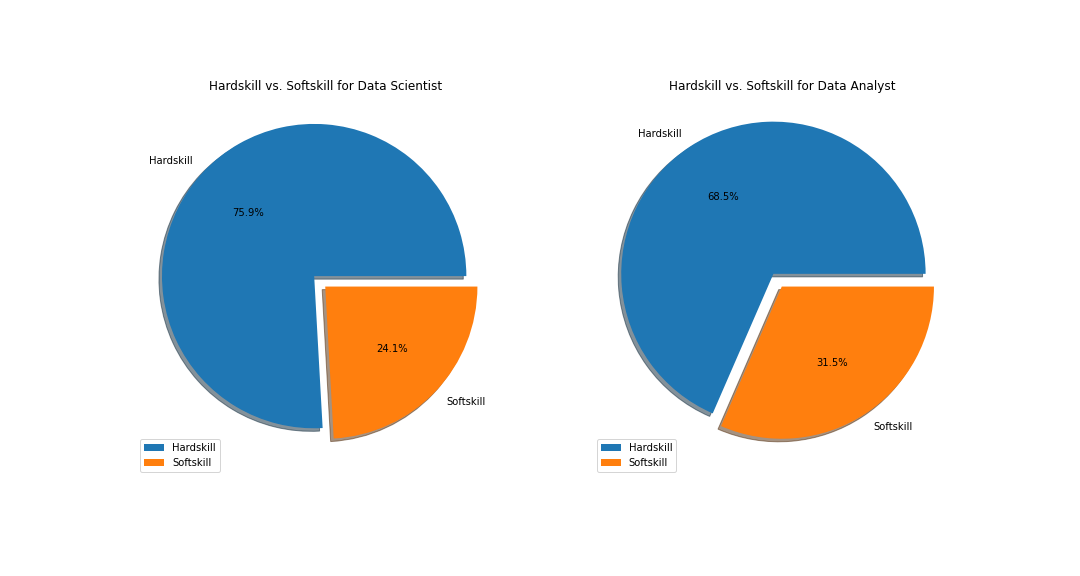
\includegraphics[width=1\textwidth]{f3.png}
  \caption{'Hardskill vs. Softskill'}
\end{figure}

\begin{figure}[H]
  \centering
  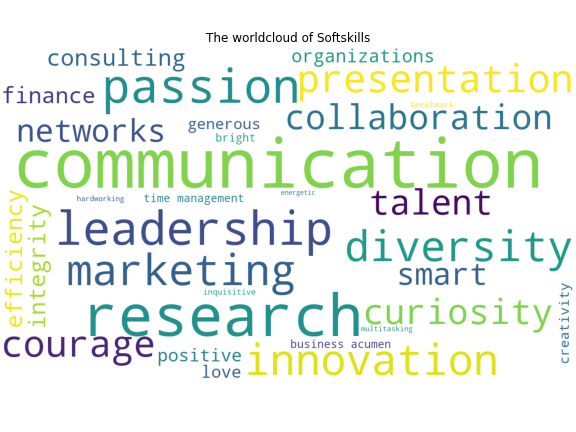
\includegraphics[width=.75\textwidth]{f1.png}
  \caption{'The Worldcloud of Soft Skills'}
\end{figure}

\begin{figure}[H]
  \centering
  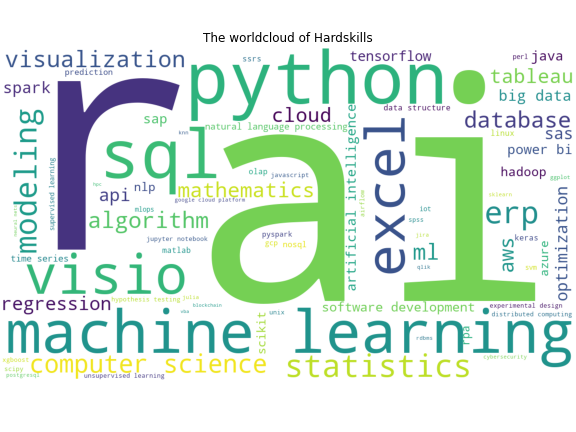
\includegraphics[width=.75\textwidth]{f4.png}
  \caption{'The Worldcloud of Hard Skills'}
\end{figure}

\begin{figure}[H]
  \centering
  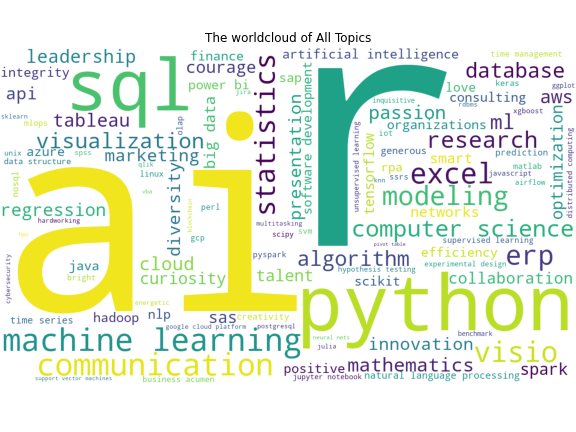
\includegraphics[width=.75\textwidth]{f5.png}
  \caption{'The Worldcloud for All Topics'}
\end{figure}

\begin{figure}[H]
  \centering
  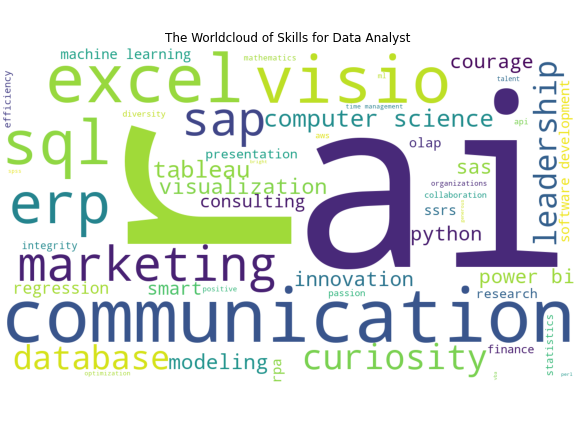
\includegraphics[width=.75\textwidth]{f7.png}
  \caption{'The Worldcloud for All Topics to DA'}
\end{figure}

\begin{figure}[H]
  \centering
  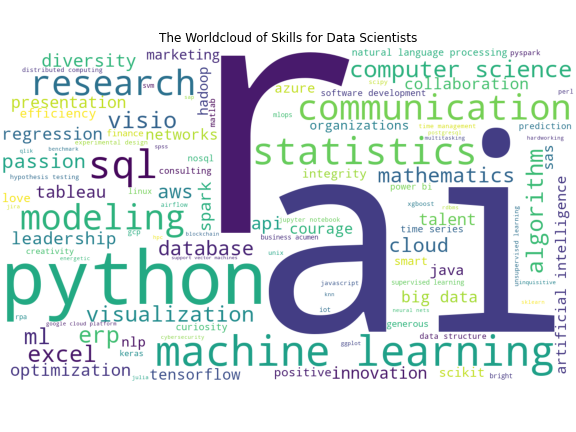
\includegraphics[width=.75\textwidth]{f6.png}
  \caption{'The Worldcloud for All Topics to DS'}
\end{figure}

\begin{figure}[H]
  \centering
  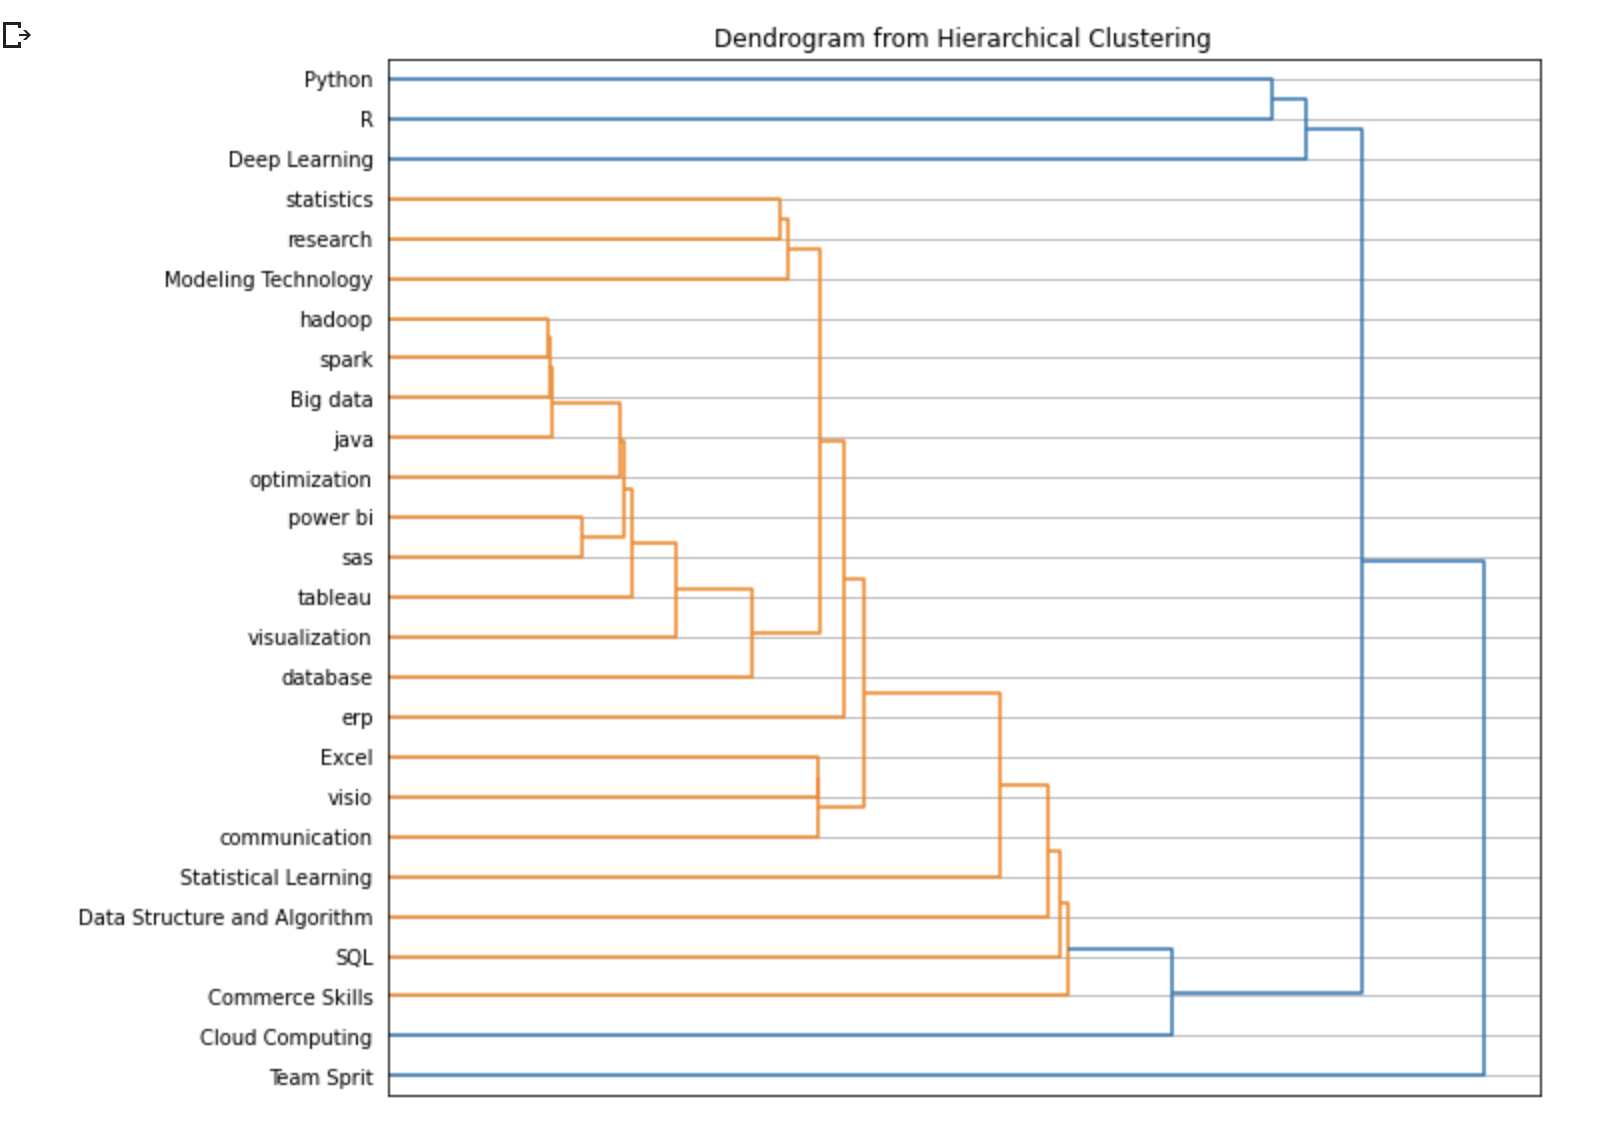
\includegraphics[width=1\textwidth]{f8.png}
  \caption{'Dendrogram from Hierarchical Clustering'}
\end{figure}

\begin{figure}[H]
  \centering
  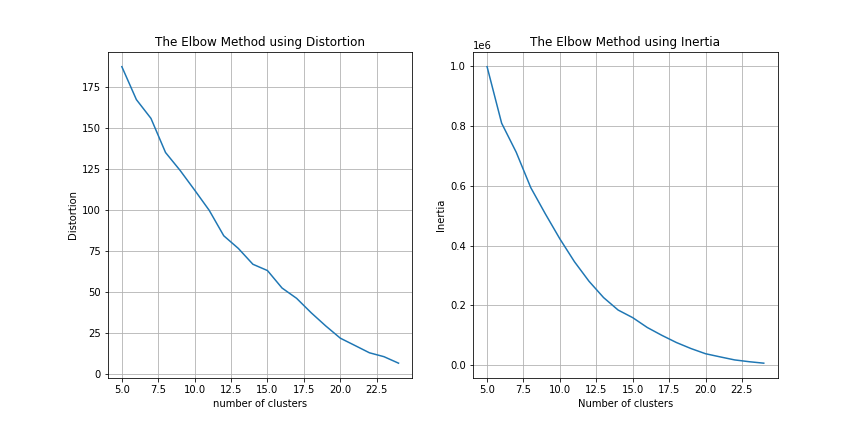
\includegraphics[width=1\textwidth]{f9.png}
  \caption{'Elbow Method Visualization'}
\end{figure}

\begin{figure}[H]
  \centering
  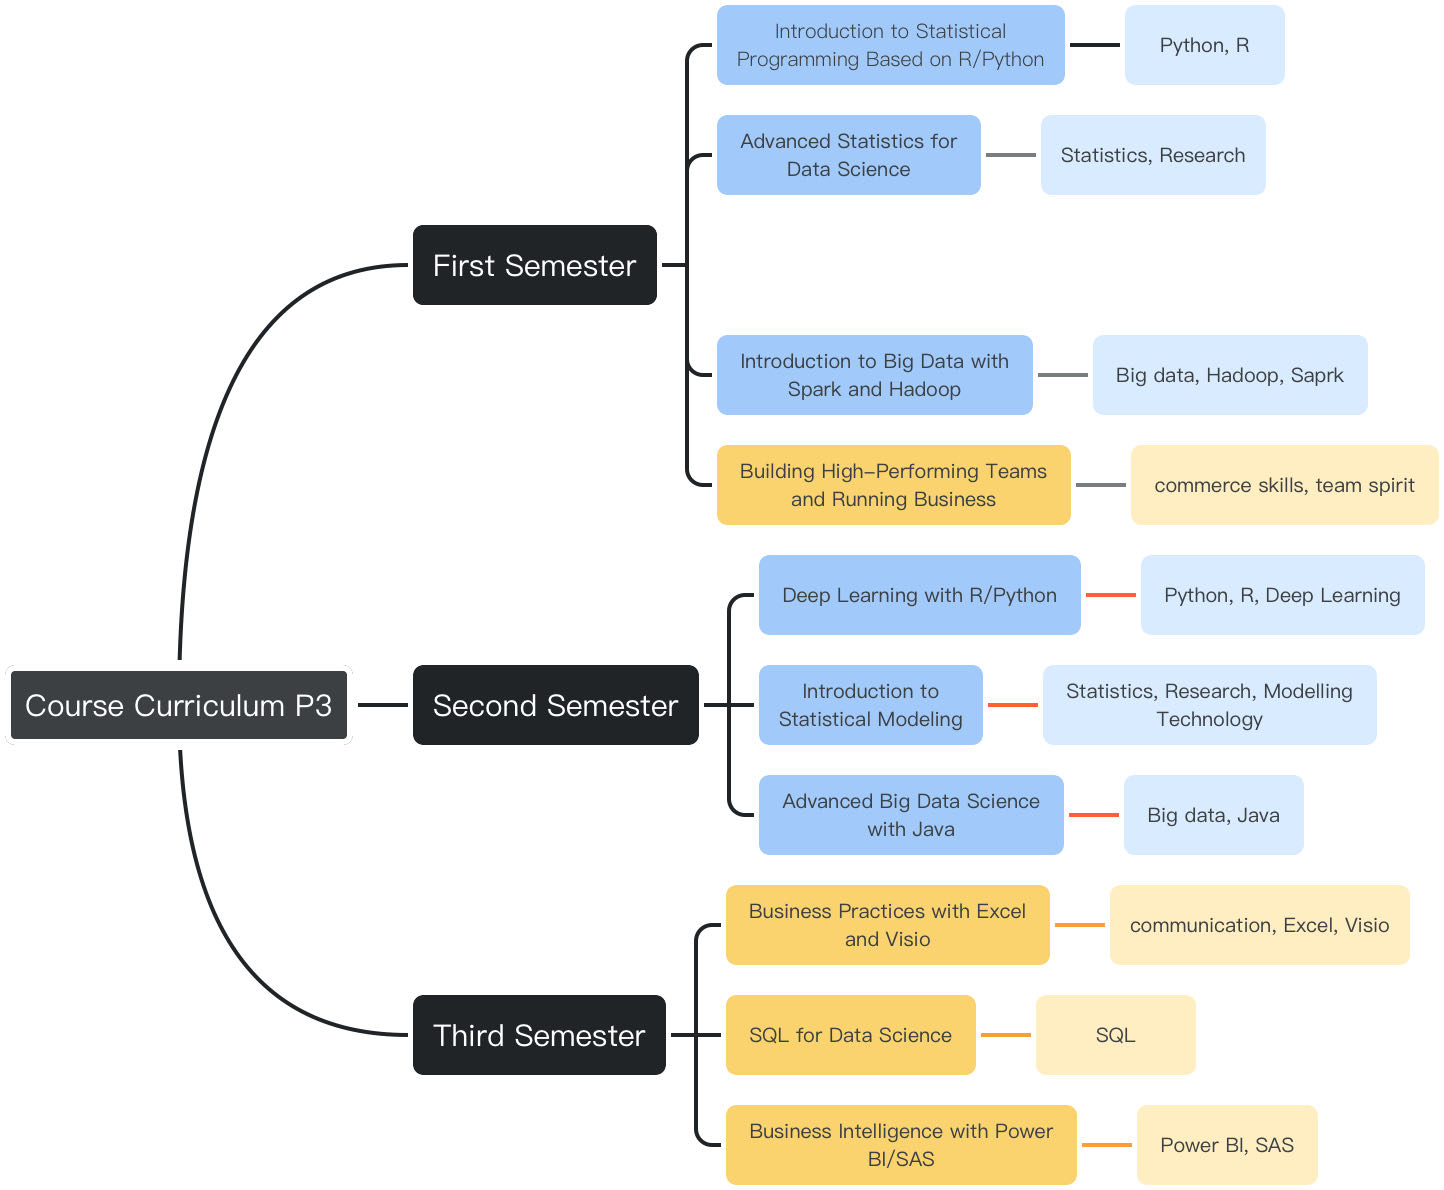
\includegraphics[width=1\textwidth]{f10.png}
  \caption{'Course Curriculum P3'}
\end{figure}

\begin{figure}[H]
  \centering
  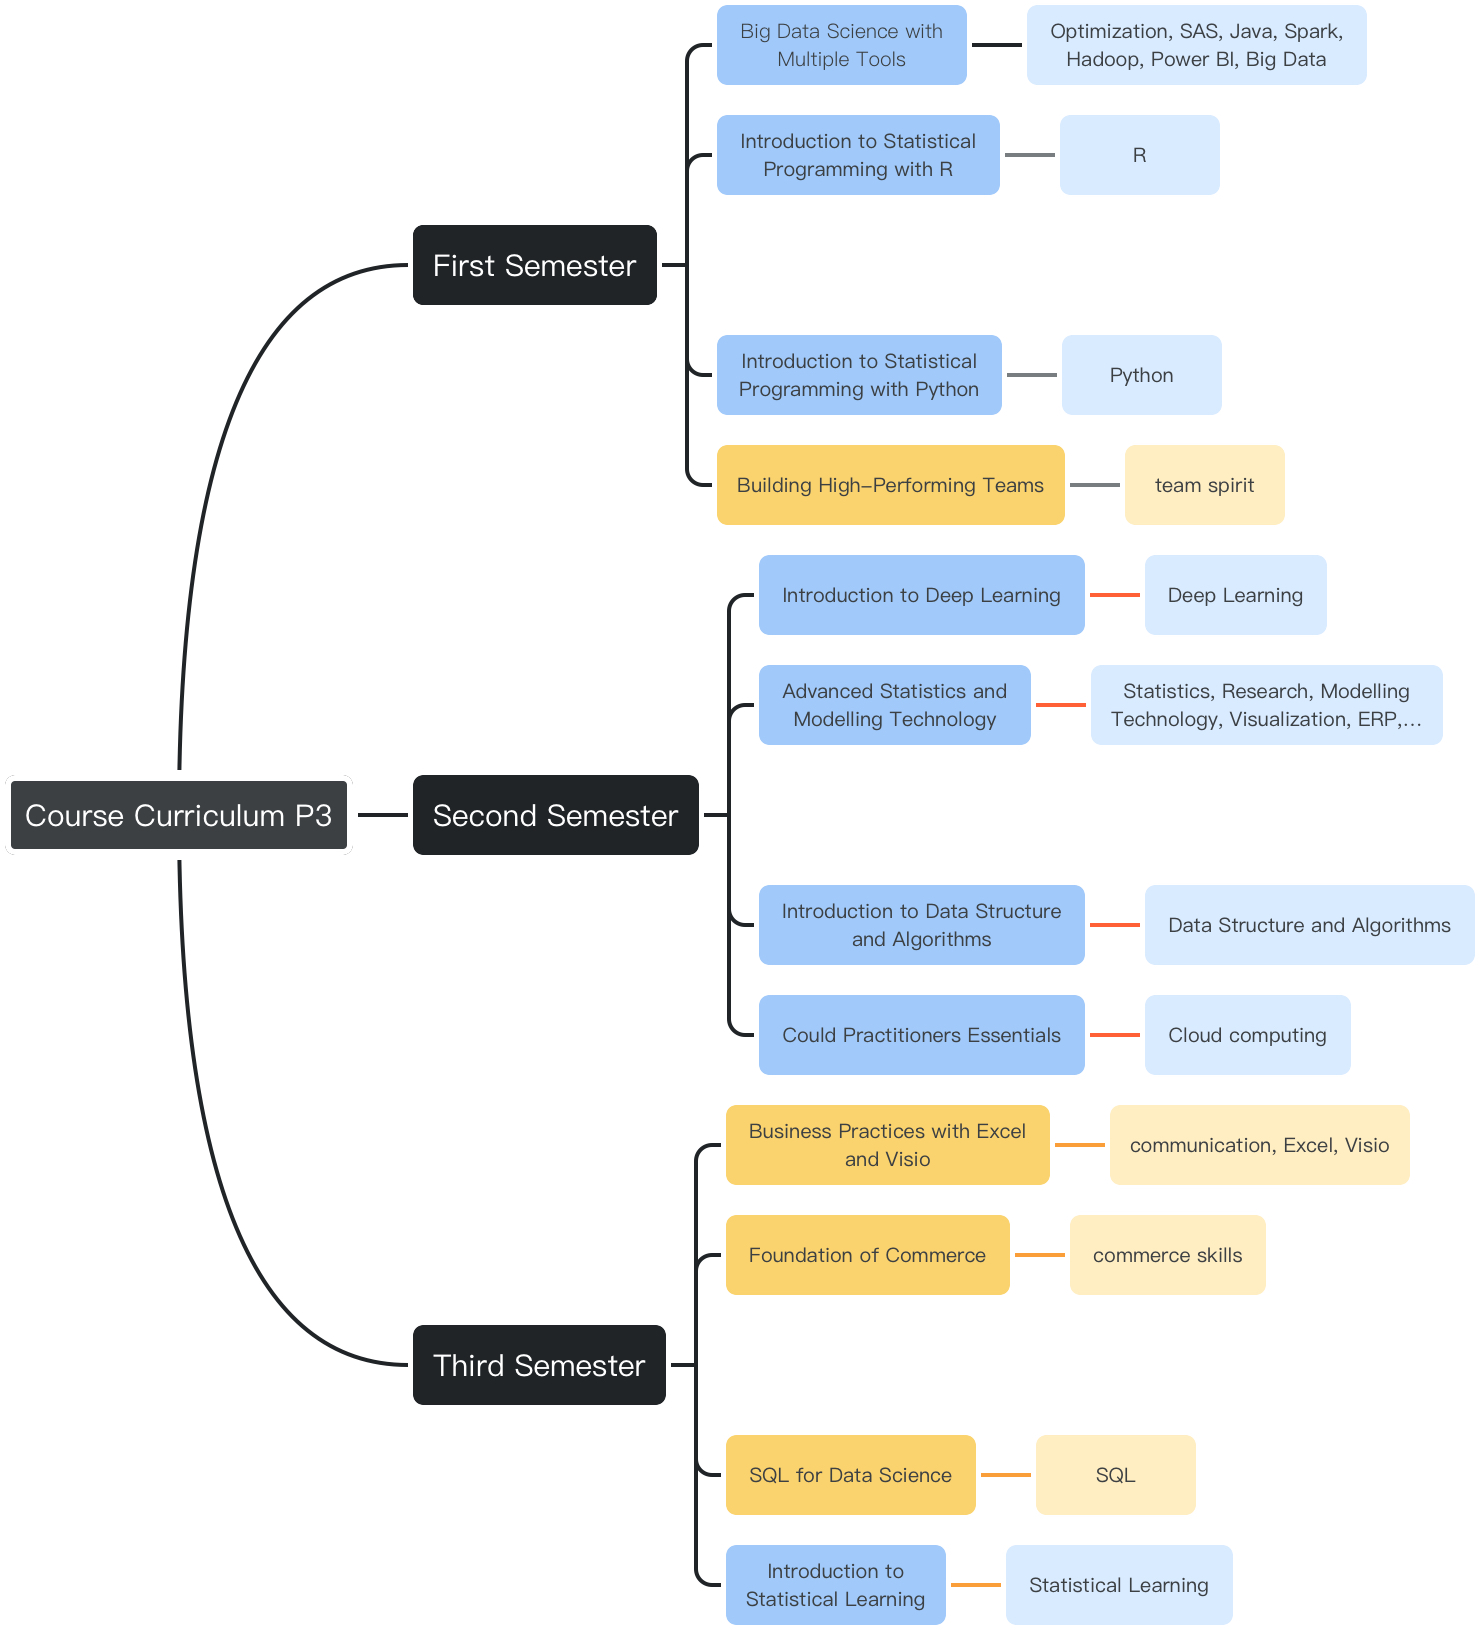
\includegraphics[width=1\textwidth]{f11.png}
  \caption{'Course Curriculum P4'}
\end{figure}

\end{document}